\chapter{Method}
\label{chap:method}
In the previous chapter different indoor localization methods were introduced. From this information an initial system design was destilled. The details of the different components can be found in the following sections.

\section{Proof of Concept System Overview}
Summarizing the information and the decision made so far, the overall proof of concept can be found in \cref{fig:system_design}.
\textcolor{cyan}{further explanation}

\begin{figure}[H]
	\centering
	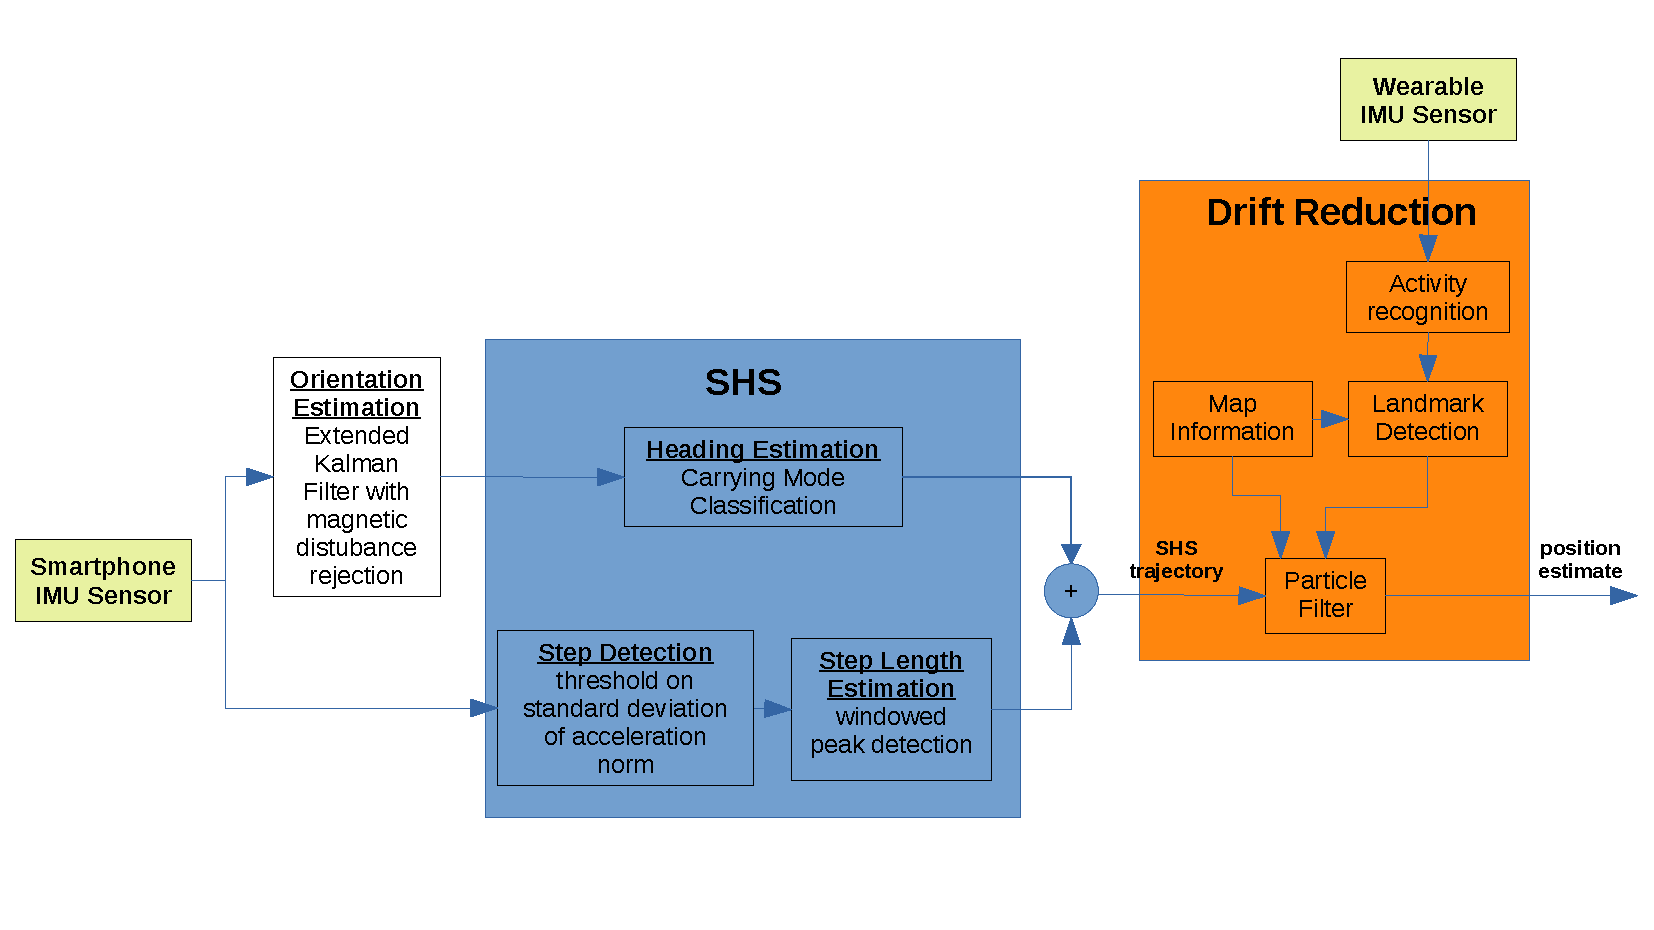
\includegraphics[width=\linewidth]{images/system_design}
	\caption{Overview of proof of concept SHS-PF with activity recognition from wearable device}
	\label{fig:system_design}
\end{figure}


\section{Step Detection and Step Length Estimation}

\textcolor{cyan}{introductory text}

\subsection*{Step Detection}
\label{sec:meth - step detection}
The method used for step detection is similar to the one presented by \cite{Salvi2018}, introduced in \secref{sec:rw - step detection}. 
 An overview of the different components of this windowed peak detection method is shown in \cref{fig:step_detection} . To optimize the algorithm, different combinations of stage components were compared in \cite{Salvi2018}. A custom made, electronic ground truth device was worn by test subjects for easy comparison with the different parameter settings. A dataset of 36 recordings was made,  where three researchers walking for two to three minutes with the phone held in six different carrying modes. This includes in hand, in a front pocket, in a back pocket, in an armband, in a shoulder purse, and in a neck pouch on a string. Each set contains around 2.5 minutes of accelerometer and ground truth data.
\begin{figure}
	\centering
	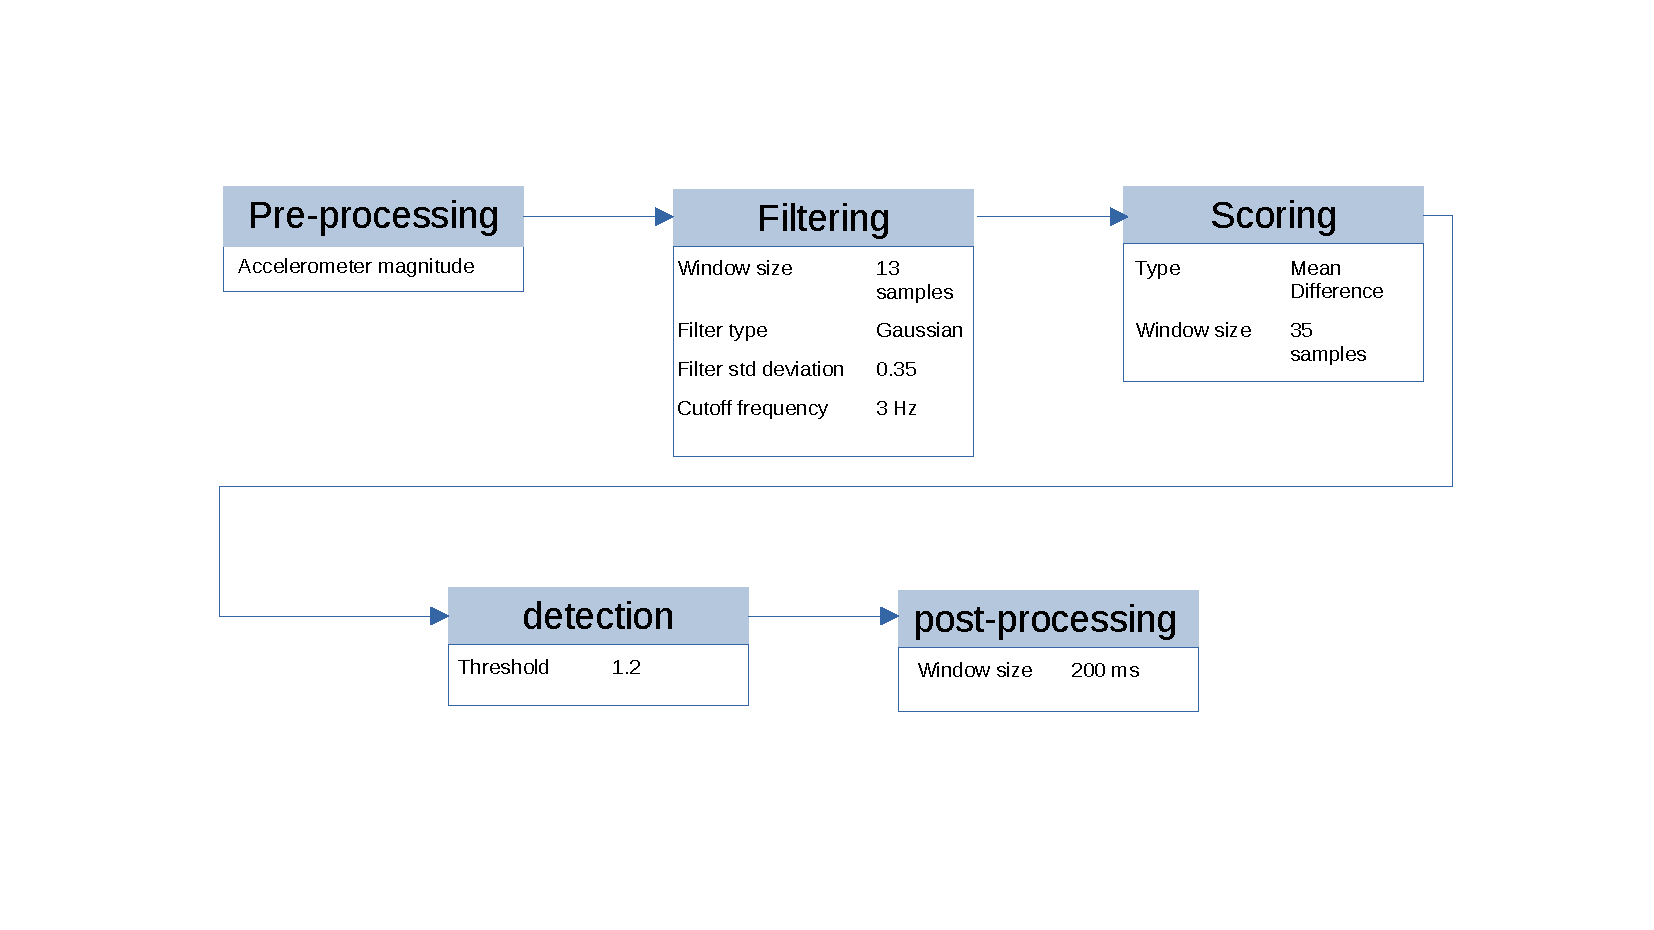
\includegraphics[trim=20 100 50 80, clip, width=0.7\linewidth]{images/step_detection}
	\caption{Windowed peak detection components and parameters used by \cite{Salvi2018}}
	\label{fig:step_detection}
\end{figure}

 This thesis uses the method and parameters found by \citet{Salvi2018} as basis for step detection. The eventually implemented method differs slightly from the referenced paper in that the data is being handled offline, not having to wait for data buffers to fill. It also differs in that it adds the walk detection method from \cite{Brajdic2013}. The values used for the different parameters are based on those found by \cite{Salvi2018}. The implemented method consists of five steps:
\begin{enumerate}
	\item \textbf{Pre-processing} \\
	The IMU used in most smartphones provide acceleration information over three orthogonal axes. For the step detection algorithm the magnitude of the combined signal from the three orthogonal axes is used.
	
	\item \textbf{Walk detection} \\
	Since a person is not walking continuously, the regions in which it does occur need to be indicated. \cite{Brajdic2013} determined that thresholding on the standard deviation of the norm the accelerometer signal was sufficient. This is done using the parameters found by the paper, which is determining the standard deviation over a moving frame of 0.8 seconds, with all standard deviation magnitude levels above $0.6 m/s^2$ being considered walking.
	
	\item \textbf{Filtering} \\
	A gaussian window is applied with a window size of 13 frames and a standard deviation of 0.35.
	
	\item \textbf{Scoring }\\
	With the scoring stage the "peakiness" of a given sample is evaluated. The result
	of this stage should increase the magnitude of any peaks. This makes it easier for the subsequent peak detection. The scoring used is that of mean difference 
	\begin{equation}
		p_{i}=\frac{\sum_{k=-N, k \neq i}^{N}\left(x_{i}-x_{i+k}\right)}{2 N}
		\label{eq:mean difference}
	\end{equation}
	where $p$ is the score given to the sample, $i$ is the index of the sample, $N$ is window size, and $x$ is the sample value.
	
	
	\item \textbf{Step detection} \\
	Here outliers are statistically detected. The algorithm processes the signal by calculating a running mean and standard deviation.
	These two measures determine whether a sample is an outlier or not. If the difference between sample and mean is over 1.2 times the standard deviation, then it is marked as a potential step.
	
	
	\item \textbf{Post-processing} \\
	The final stage of step detection is determining local maxima of the outliers detected in the previous stage. Here local maxima are found that have a minimum separation duration of 0.2 seconds.
	
\end{enumerate}

\begin{algorithm}[]
	\SetAlgoLined
	\caption{Step Detection}
	\label{algo:step_detect}
	\underline{initialization:}\\
	\For{k = 1,2,...}{
		\underline{measurement update:}\\		
	}
\end{algorithm}

The parameters used for the process coincide with those found by the researchers, an overview of which can be found in \cref{tab:parameters_used}.

\begin{table}
	\centering
	\footnotesize
	\begin{tabular}{clc} 
		\hline
		Stage & Parameters & Value \\
		\hline & Window size & $\mathrm{M}=13$ \\
		Filtering & Filter type & Gaussian \\
		& Filter SD & 0.35 \\
		\multirow{2}{*} { Scoring } & & \\
		& Type & Mean Difference \\
		& Window size & $N=35$ \\
		Detection & Threshold & 1.2 \\
		Post-Processing & $t_{\text {window}}$ & $200 \mathrm{ms}$ \\
		\hline
	\end{tabular}
	\caption{Parameters used in \cref{algo:step_detect}}
	\label{tab:parameters_used}
\end{table}

An example of this step detection method and its different stages can be found in \cref{fig:all_stages_of_step_detection}.

\begin{figure}[H]
	\centering
	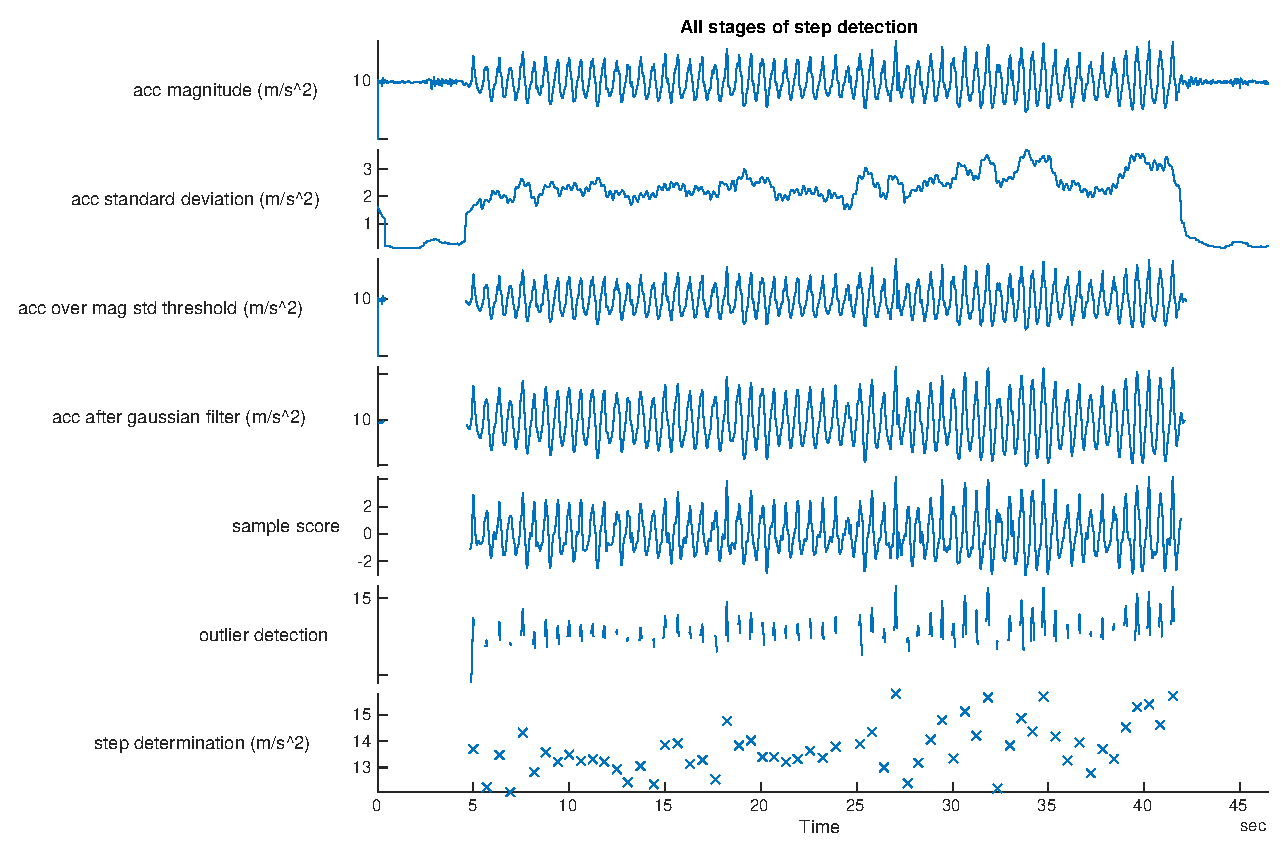
\includegraphics[width=1\linewidth]{images/20200924_1204_All_stages_of_step_detection}
	\caption[All stages of step detection ]{All stages of step detection from recorded accelerometer data, with the x's in the last graph indicating the steps taken }
	\label{fig:all_stages_of_step_detection}
\end{figure}
\subsection*{Step Length Estimation}
For step length estimation the method outlined as working best by \cite{Vezocnik2019} will be used. This is \eqref{eq:Tian2016_sle} in \cref{sec:rw-SHS}. Within this method there is a tuneable parameter that needs to be estimate in order for the method to be applied. One way of doing this is by using the data that \cite{Vezocnik2019} have made available online. Running this data through the above outlined step detection, the result can be used for parameter estimation.

\textcolor{red}{this section is pretty small at the moment, should it require a heading? What else to add?}

\section{Orientation Estimation}
\textcolor{cyan}{introductory text}
\subsection{Coordinate Frames}
Within orientation estimation there are  different coordinate frames to be considered. There are two frames that are of importance for localization: the body frame and the navigation frame.\\
The body frame ($b$) is the coordinate frame of the IMU, the origin of which is at the center of the triaxial accelerometers found in the device \cite{Kok2017}. The navigation frame ($n$) is the geographical frame in which the user is moving. It is also the frame in which we want to determine the pose, consisting of orientation and position, of the body frame. For a localization application it is considered stationary \cite{Kok2017}.
A superscript on a vector is used to indicate in which coordinate frame it is expressed. For example,
$x^n$ is the vector $x$ expressed in the navigation frame. A double superscript on any orientation mapping from one frame to another indicates from which frame to which frame the rotation is occurring. For example,
$R^{nb}$ is a rotation matrix that maps from the body frame to the navigation frame.


\subsection{Orientation Parametrization}
While position is often represented by a point in a 3D orthogonal axis frame, orientation has different parametrizations, each able to map to one another. This chapter will introduce rotation matrices ($R$) and quaternions ($q$), which will be used in the following section to determine orientation from IMU sensor data.

\subsubsection{Rotation Matrix}
Rotation matrices $R \in \mathbb{R}^{3 \times 3}$ have the following properties:

\begin{equation}
	\label{eq:rot_mat_properties}
	R R^{\top}=R^{\top} R=I_{3}, \quad \text { det } R=1.
\end{equation}

These matrices can be used to express a vector $x$ in frame $v$ to frame $u$ as 

\begin{equation}
	\label{eq:rot_mat_rot_x}
	x^{\mathfrak{u}}=R^{\mathfrak{u} \mathrm{v}} x^{\mathrm{v}}.
\end{equation}

Transposing a rotation matrix represent a rotation back to it's original coordinate frame:
\begin{subequations}
	\begin{align}
		\label{eq:rot_mat_trans}
		x^{\mathrm{v}}&=\left(R^{\mathrm{uv}}\right)^{\top} x^{\mathrm{u}},\\
		&=R^{\mathrm{vu}} x^{\mathrm{u}}.
	\end{align}
\end{subequations}

\subsubsection{Quaternion}
A quarternion is a common parametrization of orientation frequently used by attitude estimation algorithms. This is because it is free of non-singularity in attitude representation \cite{Hashim2019}, also known as wrapping. A unit quaternion can be described by

\begin{equation}
	\label{eq:unit_quarternion}
	q=\left(\begin{array}{llll}{q_{0}} & {q_{1}} & {q_{2}} & {q_{3}}\end{array}\right)^{\top}
	=\left(\begin{array}{l}{q_{0}} \\ {q_{v}}\end{array}\right), 
	\quad q \in \mathbb{R}^{4}, 
	\quad\|q\|_{2}=1.
\end{equation}

A rotation of vector $x$ using quaternions between two frames, from $v$ to $u$, is indicated as

\begin{equation}
	\label{eq:quat_rot}
	\bar{x}^{\mathrm{u}}=q^{\mathrm{uv}} \odot \bar{x}^{\mathrm{v}} \odot q^{\mathrm{vu}},
\end{equation}

where $q^{\mathrm{vu}} = \left(q^{\mathrm{uv}}\right)^{\mathrm{c}}$, with the latter representing the quaternion conjugate, defined by 

\begin{equation}
	\label{eq:quat_conjugate}
	q^{\mathrm{c}}=\left(\begin{array}{c}{q_{0}} \\ {-q_{v}}\end{array}\right).
\end{equation}

$\bar{x}^u$ represents the quaternion version of the vector $x^u \in \mathbb{R}^3$, as

\begin{equation}
	\label{eq:quat_vec_ref}
	\bar{x}^u=\left(\begin{array}{l}{0} \\ {x^u}\end{array}\right).
\end{equation}


The $\odot$ operator describes quaternion multiplication, defined by:

\begin{equation}
	\label{eq:quat_multiplication}
	p \odot q=\left(\begin{array}{c}{p_{0} q_{0}-p_{v} \cdot q_{v}} \\ {p_{0} q_{v}+q_{0} p_{v}+p_{v} \times q_{v}}\end{array}\right)
\end{equation}

\subsection{Motion and Measurement Models}
\label{sec:motion_and_measurement_models}
The signals generated by an IMU can be formatted in such a way that orientation can be deduced. For many sensor fusion algorithms this is generally done by defining a motion and measurement model, together forming a state space representation. This state space can be defined as \cite{Kok2017}

\begin{subequations}
	\begin{align}
		\label{eq:orient_dynamics}
		q_{t+1}^{\mathrm{nb}} &=q_{t}^{\mathrm{nb}} \odot \exp _{\mathrm{q}}\left(\frac{T}{2}\left(y_{\omega, t}+e_{\omega, t}\right)\right), 	\\ 
		\label{eq:orient_acc_measure}
		y_{\mathrm{a}, t} &=-R_{t}^{\mathrm{bn}} g^{\mathrm{n}}+e_{\mathrm{a}, t},\\ 
		\label{eq:orient_mag_measure}
		y_{\mathrm{m}, t} &=R_{t}^{\mathrm{bn}} m^{\mathrm{n}}+e_{\mathrm{m}, t}, 
	\end{align}
	\begin{equation}
		\label{eq:orient_ss_noise}
		e_{\omega, t} \sim \mathcal{N}\left(0, \sigma_{\mathrm{\omega}}^{2} \mathcal{I}_{3}\right), 
		\quad 
		e_{\mathrm{a}, t} \sim \mathcal{N}\left(0, \sigma_{\mathrm{a}}^{2} \mathcal{I}_{3}\right), 
		\quad 
		e_{\mathrm{m}, t} \sim \mathcal{N}\left(0, \sigma_{\mathrm{m}}^{2} \mathcal{I}_{3}\right).
	\end{equation}
	\label{eq:orient_state_space}
\end{subequations}

Here \eqref{eq:orient_dynamics} is the motion model and \eqref{eq:orient_acc_measure,eq:orient_mag_measure} are the measurement models. \\
For the motion model, $q^{nb}$ represents unit quaternion from body $(b)$ to navigation frame $(n)$. $T$ is the time period between two samples. $y_{\omega, t}$ is the gyroscope measurement. The $\odot$ operator describes quaternion multiplication, as in \eqref{eq:quat_multiplication}. The $\text{exp}_\text{q}$ operator is defined as

\begin{equation}
	\exp_\mathrm{q} (\eta) = \left(\begin{array}{c}{\cos \|\eta\|_{2}} \\ {\frac{\eta}{\|\eta\|_{2}} \sin \|\eta\|_{2}}\end{array}\right) \label{eq:exp_q_in_text}.
\end{equation}

For the measurement model, $y_{\mathrm{a}, t}\in \mathbb{R}^3$ is the accelerometer measurement and $R^\mathrm{nb}_t$ is the rotation matrix mapped from the orientation quaternion generated in \eqref{eq:orient_dynamics}. $g^n \in \mathbb{R}^3$ is the gravity vector in the navigation frame. Similarly, $y_{\mathrm{m}, t}\in \mathbb{R}^3$ is the accelerometer measurement and $m^n$ is the magnetic field in the navigation frame. \\
This state space model is simplified using certain assumptions.
For both motion and measurement models, the noise terms  $(e)$ is assumed to be normally distributed, independent and have the same noise levels for the three sensor axis of all three sensors, as indicated in \eqref{eq:orient_ss_noise}. The zero mean in these noise definitions also indicate the assumption that the sensors have been calibrated properly and therefore do not contain any bias. \\
Another assumption is that the sensor does not travel over significant distances in comparison to the size of the earth \cite{Kok2017}. Additionally the magnitude of the earth rotation and coriolis acceleration are discarded. Furthermore, it is assumed that the acceleration signal is dominated by the gravity vector, making external acceleration negligible. Additionally, the magnetic field is assumed to be constant. These different assumptions will be needed to taken into account when constructing orientation estimation while walking indoors.

\subsection{Calibration}

For proper orientation estimation, sensor calibration is required. \\
\textcolor{cyan}{elaboration need to introduce the subject} 

%\citet{Moder2017} indicates that it is  beneficial for PDR systems to have the gyroscope and magnetometer bias  calibrated, while the accelerometer bias and scale factor is optional. In addition it is advised to estimate the gyroscope bias frequently before testing.

\subsubsection{Gyroscope Calibration}
Gyroscope measurements from MEMS IMUs are generally offset by a bias ($o_\omega$) and influenced by noise ($e_{\omega, t}$)  resulting in

\begin{equation}
	y_{\omega, t}=\omega_{t}+o_{\omega}+e_{\omega, t},
\end{equation}

where $e_{\omega, t}$ is assumed to have the same noise properties as in \eqref{eq:orient_ss_noise}. The gyroscope bias is slowly time varying but for relatively short experiments can be assumed to be constant \cite{Kok2016}. It can be measured by placing the gyroscope on a flat surface for some time and recording data from the sensor. Since the sensor is not moving, the biases are the means of the data over the three axis and the covariance is the square of the standard deviation of the data to the previously mentioned means.

\subsubsection{Accelerometer and Magnetometer Calibration}
% In outdoor environments, mn is equal to the local earth magnetic field and is accurately
%known from geophysical studies, see e.g. [29]. In indoor environments, however, the local magnetic
%field can differ quite significantly from the local earth magnetic field. Because of that, we treat mn as
%an unknown constant. 

For magnetometer and accelerometer calibration the method outlined by \citet{Kok2016} can be used. This method indicates that for a perfect calibration a magnetometer measures the local magnetic field, no matter the orientation. Any measurement will then lie on a sphere with a radius  equal to the local magnetic field. The same applies for a perfect calibration with an accelerometer, replacing the local magnetic field with the gravity vector. Any sensor calibration should strive to achieve this sphere as best as possible.\\
MEMS sensor are imperfect sensors, with sensor specific errors that can differ per sensor. These errors, including non orthogonality of sensor axis, the presence of zero bias, and difference in sensitivity on different axis \cite{Kok2016} can be combined into a distortion matrix $D$ and offset vector $o$.
This results in the following uncalibrated measurement model,
\begin{equation}
	y_{\mu, t}=D_\mu R_{t}^{\mathrm{bn}} \mu^{\mathrm{n}}+o_\mu +e_{\mu, t},
\end{equation}

where $\mu$ is a placeholder for either the acceleration vector or local magnetic field vector with the superscript indicating in what coordinate frame it is expressed. Each have their own respective distortion matrix and offset vector. $y_{\mu, t}$ represents the measurement associated with either gyroscope or magnetometer.
Due to the distortion matrix and offset vector, the measurements lie on a translate ellipsoid instead of on a sphere as previously stated. Determining these parameters, the sensor errors can be compensated through

\begin{equation}
	y_{\mu, t}^{cal}=D_\mu^{-1}\left(y_{\mu, t}-o_{\mu}\right)
\end{equation}

Without loss of generality the desired sphere radius can be normalized and written as followed to expressed the sphere characteristic
\begin{equation}
	\begin{aligned}
		\left\|\mu^{\mathrm{b}}\right\|_{2}^{2}-1 &=\left\|R_{t}^{\mathrm{bn}} \mu^{\mathrm{n}}\right\|_{2}^{2}-1 \\
		&=\left\|D^{-1}\left(y_{\mu, t}-o-e_{\mu, t}\right)\right\|_{2}^{2}-1=0.
	\end{aligned}
\end{equation}

Since real calibration measurements are still corrupted by noise, the above equality does not hold exactly. The ellipsoid fitting problem can be rewritten as

\begin{equation}
	\label{eq:calib_elipsoid}
	y_{\mu, t}^{\top} A y_{\mu, t}+b^{\top} y_{\mu, t}+c \approx 0,
\end{equation}
where
\begin{subequations}
	\label{eq:calib_elipsoid_components}
	\begin{align}
		A \triangleq D_\mu^{-\top} D_\mu^{-1}, \\
		b \triangleq-2 o_\mu^{\top} D_\mu^{-\top} D_\mu^{-1}, \\
		c \triangleq o_\mu^{\top} D_\mu^{-\top} D_\mu^{-1} o_\mu.
	\end{align}
\end{subequations}

Assuming that $A$ is positive definite, this defines an ellipsoid with parameters $A, b$ and $c$. This can be rewritten as a linear relation as

\begin{equation}
	M \xi \approx 0
\end{equation}
with
\begin{equation}
	M=\left(\begin{array}{ccc}
		y_{\mu, 1} \otimes y_{\mu, 1} & y_{\mu, 1} & 1 \\
		y_{\mu, 2} \otimes y_{\mu, 2} & y_{\mu, 2} & 1 \\
		\vdots & \vdots & \vdots \\
		y_{\mu, N} \otimes y_{\mu, N} & y_{\mu, N} & 1
	\end{array}\right), \quad \xi=\left(\begin{array}{c}
		\mathrm{vec} A \\
		b \\
		c
	\end{array}\right),
\end{equation}

where $\otimes$ is the kronecker product and vec the vectorization operator.
The ellipsoid fitting problem can be written as the following semidefinite program \cite{Kok2016} 
\begin{equation}
	\begin{array}{ll}
		\min _{A, b, c} & \frac{1}{2}\|M\left(\begin{array}{c}
			\operatorname{vec} A \\
			b \\
			c
		\end{array}\right)\|_{2}^{2} \\
		\text { s.t. } & \operatorname{Tr} A=1, \quad A \in S_{++}^{3 \times 3}
	\end{array},
\end{equation}

where $S_{++}^{3 \times 3}$ is the set of $3 \times 3$ positive definite symmetric matrices. This is a convex optimization problem with a globally optimal solution that can be solved using software packages such as CVX \cite{cvx} and YALMIP \cite{Lofberg2004}. Initial estimates of the calibration matrix $D_\mu$ and offset vector $o_\mu$ can be obtained from the estimated $\widehat{A}, \widehat{b}, \widehat{c}$ defined as

\begin{subequations}
	\begin{align}
		\beta &=\left(\frac{1}{4} \hat{b}^{\top} \widehat{A}^{-1} \widehat{b}-\widehat{c}\right)^{-1} \\
		\widetilde{D}_{\mu 0}^{\top} \widetilde{D}_{0} &=\beta \widehat{A}^{-1} \\
		\widehat{o}_{\mu 0} &=\frac{1}{2} \widehat{A}^{-1} \widehat{b}
	\end{align}
\end{subequations}

An example of this calibration can be found in \cref{fig:calibration_magnetometer} where data was recorded by recording a smartphone in as many orientations as possible, in a stationary setting. It clearly shows how the uncalibrated data is mapped to a unit sphere. The distortion matrix and offset vector for this calibration are 

\begin{subequations}
	\begin{align}
	\widehat{D}_{m0} &= \left(\begin{array}{rrr}
		0.0203 & -0.0001 & -0.0009 \\
		0 & 0.0191 & 0.0000 \\
		0 & 0 & 0.0199
	\end{array}\right), \\
	\widehat{o}_{m0} &= \left(\begin{array}{r}
		-13.3918 \\
		81.0407 \\
		20.9336
	\end{array}\right).
	\end{align}
	
\end{subequations}

\begin{figure}[H]
	\centering
	\begin{subfigure}[t]{.4\textwidth}
		\centering
		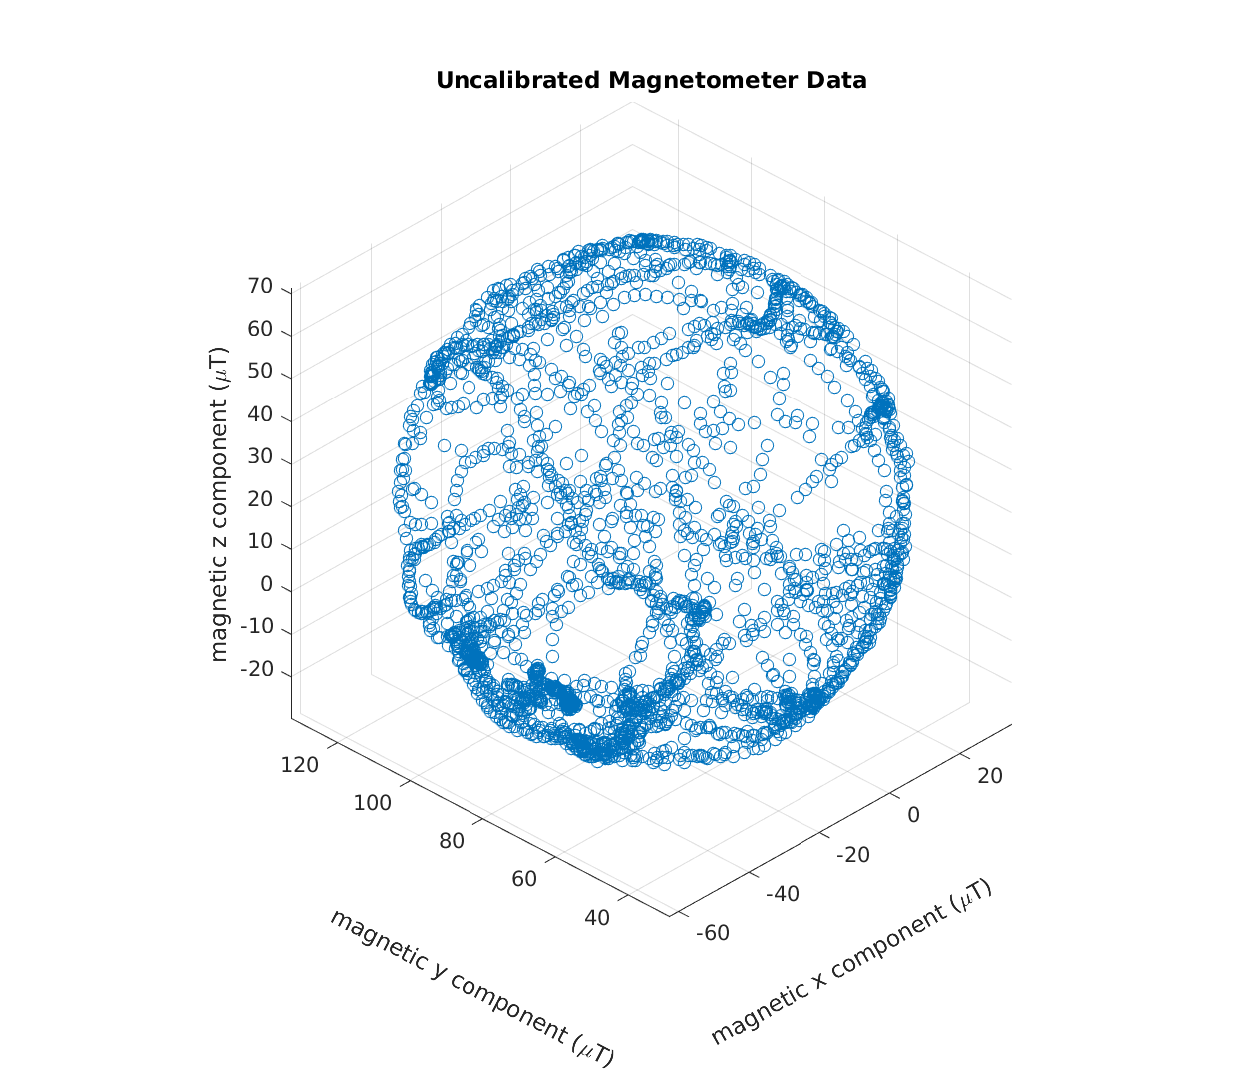
\includegraphics[width=\linewidth]{images/20201020_1125_Uncalibrated_Magnetometer_Data}
		\caption{Uncalibrated magnetometer data}
		\label{fig:uncalibrated_magnetometer_data}
	\end{subfigure}
	\begin{subfigure}[t]{0.4\textwidth}
		\centering
		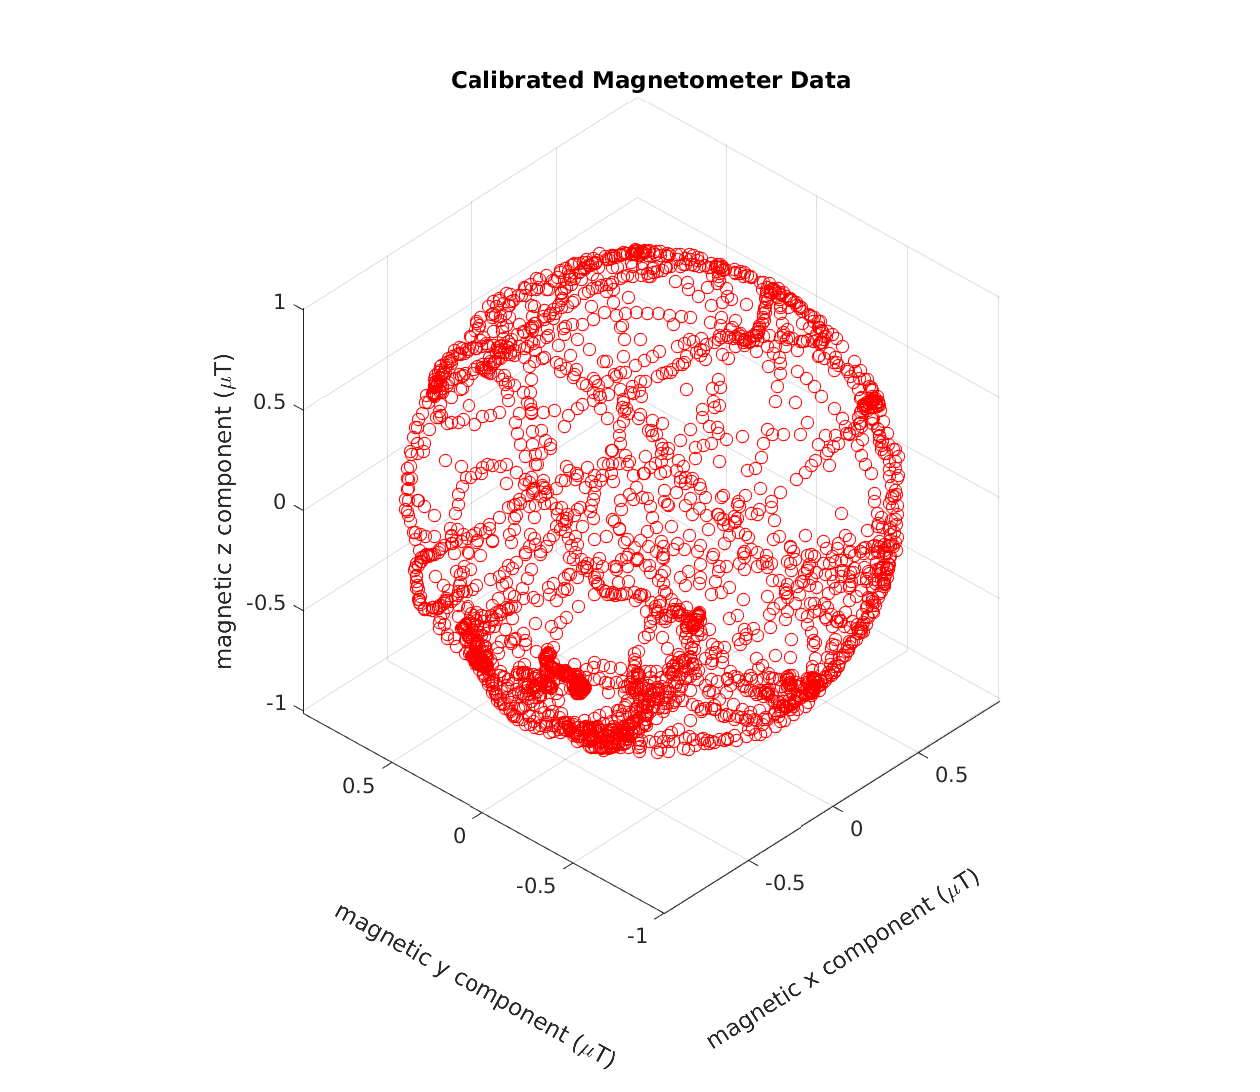
\includegraphics[width=\linewidth]{images/20201020_1125_Calibrated_Magnetometer_Data}
		\caption{ Calibrated magnetometer data}
		\label{fig:calibrated_magnetometer_data}
	\end{subfigure}
	\caption{Magnetometer calibration for smart MEMS IMU in one location}
	\label{fig:calibration_magnetometer}
\end{figure}

\newpage
\subsection{Extended Kalman Filter}
\label{sec:method-EKF}
The Kalman Filter (KF) uses a linear state space model in combination with measurements and its characteristics to make an unbiased minimum-variance estimator \cite{verhaegen2007filtering}. The KF assumes that the noise affecting the state space model is additive and that both process and measurement noise are Gaussian and zero mean.
The Kalman Filter consists of three steps, with the last two steps performed recursively. The first is stating an initial estimate and the variance of the process and measurement noise.  The second is the time update in which the state is propagated through a motion model, which may or may not have an external input, resulting in a one step ahead estimate. The third step is the measurement update in which the estimate generated by the time update is compared with actual measurements related to the state being estimated. Discrepancies between the two will lead to an error measurement. This error can then be used to correct the estimate.
The Extended Kalman Filter (EKF) is an adaptation of the Kalman Filter that estimates for non linear models. 

For orientation estimation the motion and measurement model presented in \eqref{eq:orient_state_space} can be used. As stated in \cref{sec:motion_and_measurement_models}, this model has assumptions that need to be accommodated. This will have to be incorporated in the EKF. Additionally sensor data does not all arrive at the same time. This means that the measurement update will potentially need to only update with either magnetometer or accelerometer data.  

\subsubsection{Time Update}

A time update occurs every time a gyroscope measurement ($y_\omega$) is received. It calculates a one step ahead estimate of the state vector and its covariance matrix. The calculations are as followed: 

\begin{subequations}
\begin{align}
\hat{q}_{t | t-1}^{\mathrm{nb}}=\hat{q}_{t-1 | t-1}^{\mathrm{nb}} \odot \exp _{\mathrm{q}}\left(\frac{T}{2} y_{\omega, t-1}\right) \\
P_{t | t-1}=F_{t-1} P_{t-1 | t-1} F_{t-1}^{\top}+G_{t-1} Q G_{t-1}^{\top}
\end{align}
with $Q = \Sigma_\omega$ and $P$ the state covariance. Here
\begin{align}
F_{t-1}&=\left(\exp _{q}\left(\frac{T}{2} y_{\omega, t-1}\right)\right)^{R},\\
G_{t-1}&=-\frac{T}{2}\left(\hat{q}_{t-1 | t-1}^{\mathrm{nb}}\right)^{L} \frac{\partial \exp _{q}\left(e_{\omega, t-1}\right)}{\partial e_{\omega, t-1}},
\end{align}
\end{subequations}
where $q^L$ and $q^R$ are defined as 
\begin{subequations}
\begin{equation}
q^L = \left(\begin{array}{cc}{q_{0}} & {-q_{v}^{\top}} \\ {q_{v}} & {q_{0} \mathcal{I}_{3}+\left[q_{v} \times\right]}\end{array}\right),
\end{equation}	
\begin{equation}
q^R = \left(\begin{array}{cc}{q_{0}} & {q_{v}^{\top}} \\ {-q_{v}} & {q_{0} \mathcal{I}_{3}+\left[q_{v} \times\right]}\end{array}\right).
\end{equation}
\end{subequations}

\subsubsection{Measurement Update}

A measurement update occurs every time either an accelerometer or magnetometer reading is received. \\
To ensure that the assumptions of the gravity vector being dominant in the accelerometer and the homogeneous magnetic field being dominant in the magnetometer, thresholds can be used. This is of importance with pedestrian dead reckoning, as a walking motion will induce additional external forces, affecting the acceleration measured by the IMU. Additionally, when localizing indoors, magnetic disturbance within the built environment will affect the magnetometer readings.\\
The measurement update for the EKF with quaternions as states is as followed:

\begin{subequations}
	\begin{align}
	\tilde{q}_{t | t}^{\mathrm{nb}} &=\hat{q}_{t | t-1}^{\mathrm{nb}}+K_{t} \varepsilon_{t}, \\
	\tilde{P}_{t | t} &=P_{t | t-1}-K_{t} S_{t} K_{t}^{\top}
	\end{align},
	with	
	\begin{align}
	\varepsilon_{t} &= y_{t}-\hat{y}_{t | t-1},\\
	\quad S_{t} &= H_{t} P_{t | t-1} H_{t}^{\top}+R, \\
	\quad K_{t} &= P_{t | t-1} H_{t}^{\top} S_{t}^{-1}.
	\end{align}
\label{eq:quat_meas_update}	
\end{subequations}


If an accelerometer measurement is received and whos magnitude falls in an interval around the magnitude , the variables to use in \eqref{eq:quat_meas_update} are

\begin{subequations}
	\begin{align}
	y_{t}&=
	y_{\mathrm{a}, t}, \\
	\hat{y}_{t | t-1}&=
	-\hat{R}_{t | t-1}^{\mathrm{bn}} g^{\mathrm{n}},\\
	H_{t}&=	-\left.\frac{\partial R_{t | t-1}^{\mathrm{bn}}}{\partial q_{t | t-1}^{\mathrm{nb}}}\right|_{{q_{t | t-1}^{\mathrm{nb}}}=\hat{q}_{t | t-1}^{\mathrm{nb}}} \quad g^{\mathrm{n}}.
	\end{align}
\end{subequations}

Likewise if a magnetometer measurement arrives and meets the threshold requirement, the variables are defined as

\begin{subequations}
	\begin{align}
	y_{t}&=	y_{\mathrm{m}, t},\\
	\hat{y}_{t | t-1}&=	\hat{R}_{t | t-1}^{\mathrm{bn}} m^{\mathrm{n}},\\
	H_{t}&=	\left.\frac{\partial R_{t | t-1}^{\mathrm{bn}}}{\partial q_{t | t-1}^{\mathrm{nb}}}\right|_{{q_{t | t-1}^{\mathrm{nb}}}=\hat{q}_{t | t-1}^{\mathrm{nb}}} \quad m^{\mathrm{n}}.
	\end{align}
\end{subequations}

\subsubsection{Renormalization}
Once a measurement update occurs the resulting quaternion is not necessarily a unit quaternion, which is a requirement for orientation parametrization. To facilitate this a renormalize the quaternion is required, using

	\begin{equation}
	\hat{q}_{t | t}^{\mathrm{nb}}=\frac{\tilde{q}_{t-1}^{\mathrm{nb}}}{\left\|\tilde{q}_{t | t}^{\mathrm{nb}}\right\|_{2}}.
	\end{equation}

Using steps outlined in \cite{Kok2017} and \cite{Linkoping2013}, the above outlined EKF was implemented in MATLAB. It was preliminarily  tested in a limited case with actual smartphone sensors. Calibration and testing occurred in the same room, where the phone was continuously randomly orientated while recording sensor data. This data was afterwards exported and entered into the EKF. The results can be seen in \cref{fig:simple_stationary_ekf}, where it is compared with the orientation estimation calculated by the android system. It is clear that the orientation estimation is almost identical to the system derived orientation.

\begin{figure}[H]
	\centering
	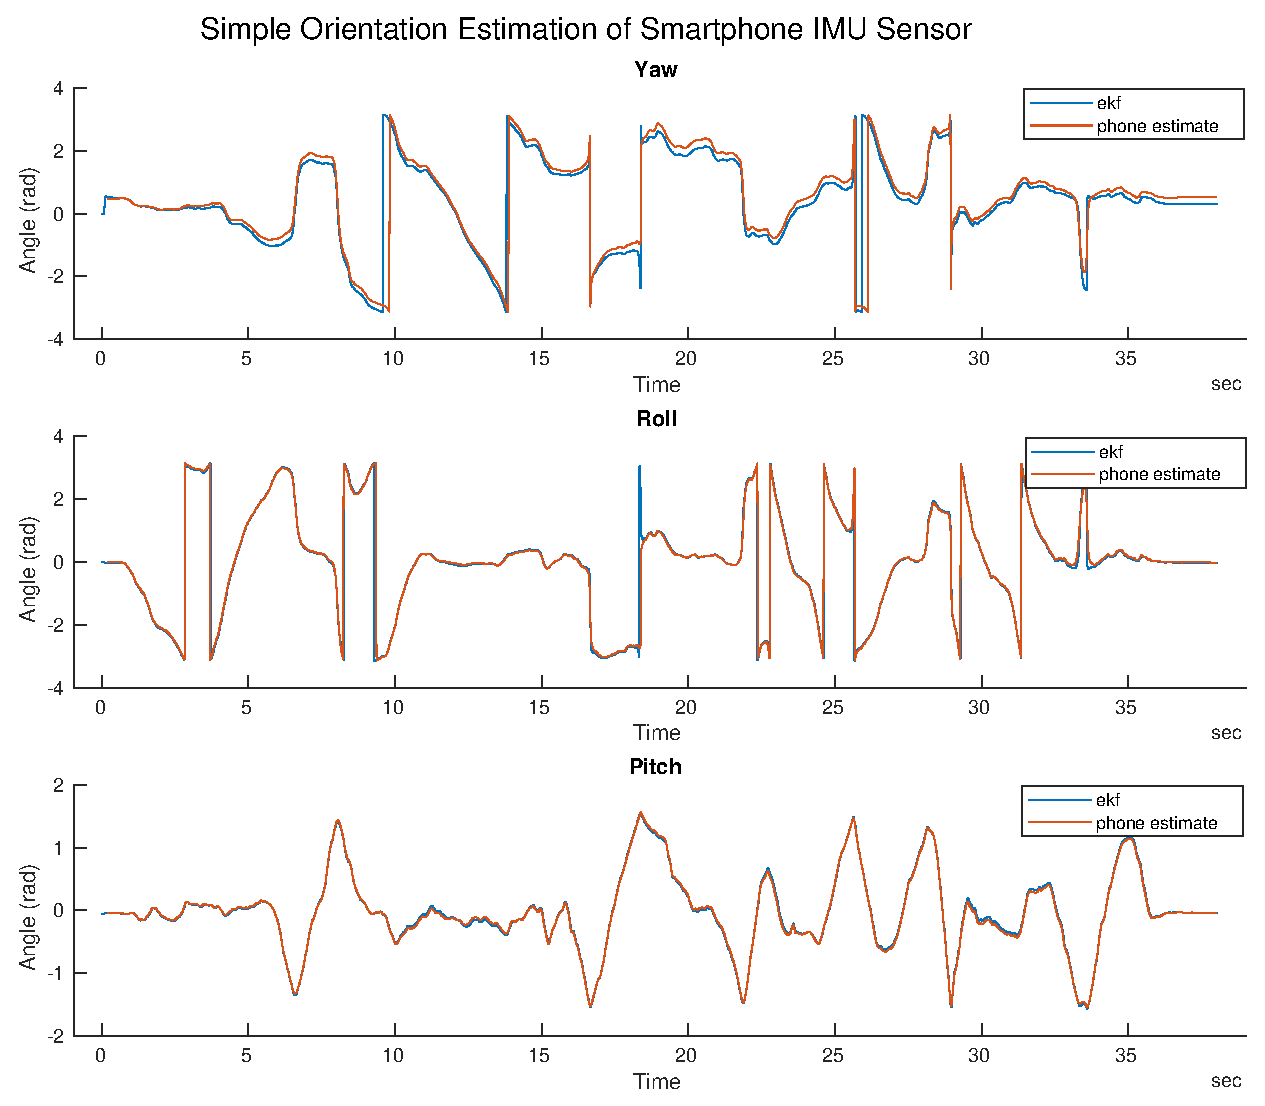
\includegraphics[width=0.7\linewidth]{images/20201025_2015_simple_stationary_ekf}
	\caption[Simple orientation estimation comparison]{ Simple orientation estimation comparison between own EKF and android orientation estimation}
	\label{fig:simple_stationary_ekf}
\end{figure}

\textcolor{red}{what other metrics are important to show to proof the performance of the EKF?}

\newpage
\section{Map based Particle Filter with Landmark Measurement Update}
In \cref{sec:rw-drift_reduction}, the Particle Filter was introduced as a drift reduction method able to handle spatial context such as map information, landmarks and spatial models. In this section, the spatial information of the experimental setup is shown and the implementation of the particle filter with step and heading system input is presented.

\subsection*{Map Creation}
In order to use spatial context with the particle filter, different sources were combined to generate a map of the experiment space. Rudimentary blueprints of the building were used generate a diagram of the indoor environment. The positioning and size of furniture was estimated. The resulting image has clear color distinction between the different structures within the building, including walls, doors and furniture, as seen in \cref{fig:indoor_blueprint}. Through a comparison between structures in the generated image and satellite images, shown in \cref{fig:house_google_maps}, the image was transformed from pixel to meter coordinates. This provides the basis for incorporating spatial context within a Particle Filter.

\begin{figure}[H]
	\centering
	\begin{subfigure}[t]{.38\textwidth}
		\centering
		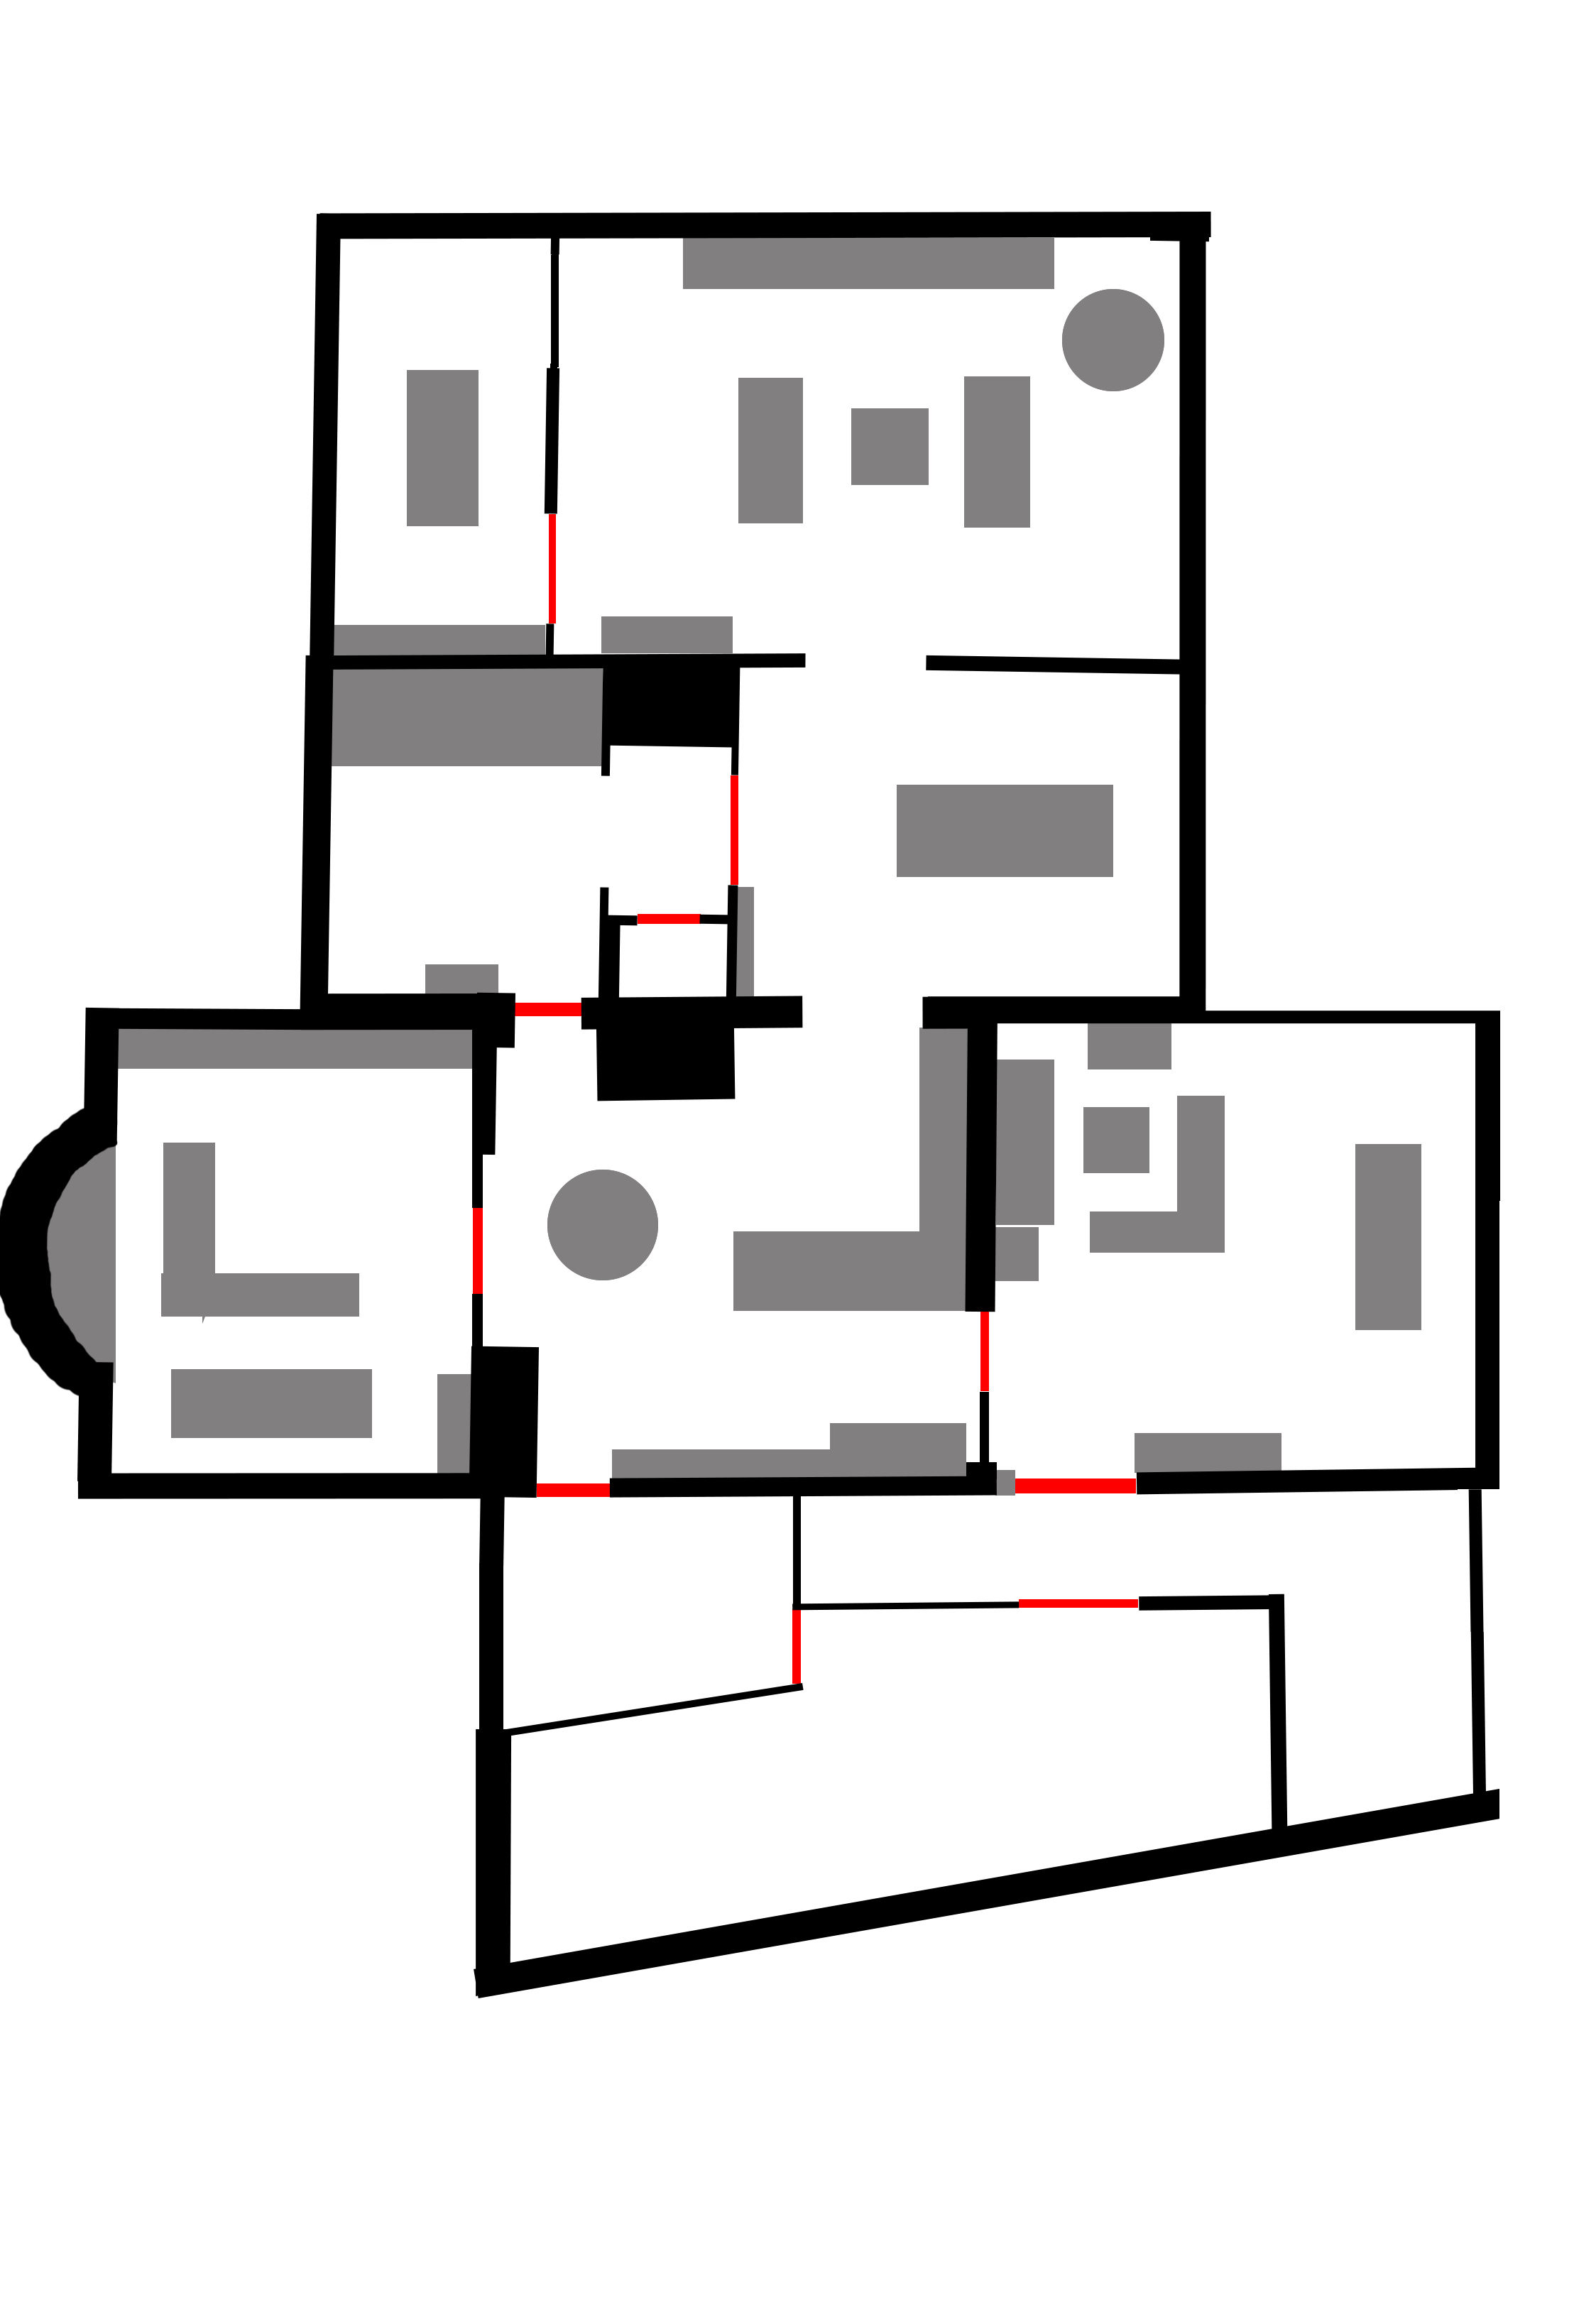
\includegraphics[width=0.9\linewidth]{images/indoor_blueprint}
		\caption[Image from building blueprints]{Image from building blueprints. Black, grey and red represent walls, furniture, and doors, respectively.}
		\label{fig:indoor_blueprint}
	\end{subfigure} \quad
	\begin{subfigure}[t]{.4\textwidth}
		\centering
		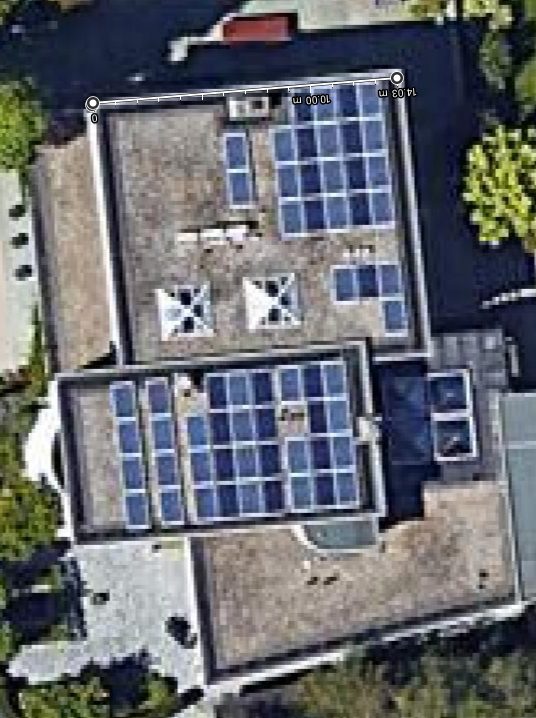
\includegraphics[width=0.9\linewidth]{images/house_google_maps}
		\caption{Measurement from Google Maps}
		\label{fig:house_google_maps}
	\end{subfigure} \quad
	\label{fig:particle_map_construction}
	\caption{Particle filter map creation}
\end{figure}

\subsection*{Implementation}

The implementation of the particle filter for indoor localization using SHS trajectory and activity recognition as input will be explained next.  \cref{algo:bootstrap_PF} summarizes the whole approach.

\subsubsection*{Initialization}
For indoor localization on one floor, particles are limited to $\mathbb{R}^{2}$ and by the outer perimeter of the building the user is located in. The particle is defined by 

\begin{equation}
x_k^i = \left(\begin{array}{l}
p_{1,k}^i   \\
p_{2,k}^i  \\
\theta_k^i
\end{array}\right), 
\label{eq:pf_state}
\end{equation}
where $x^i_k$ is the state of particle $i$ at time $k$, $p_1 $ and $p_2$ are the particle x axis and y axis position respectively. The heading angle is  $\theta$.\\
For initialization,  all particles are positioned around a known starting point. The initial weight of each particle $\omega^i$ is $1/N$, where $N$ is the total number of particles. Once initialized the following three steps are performed recursively \cite{Wu2019,Woodman2008}: 

\begin{enumerate}
	\item \textbf{Measurement update} \\
	There are two measurement updates possible within the particle filter, one that compares particle trajectories to map constraints and the other were door positions are compared with particle positions. \par 
	
   With a map, the position of physical structures can be compared with the trajectory of particles as a measurement update. If these structures cannot be traversed, as is the case with walls, the trajectory of a particle that crosses such a structure is incorrect. This makes the likelihood of it being a position estimate 0, rendering its weight 0 as well. Particles that traverse accessible regions have a likelihood of 1, and therefore also a weight of 1. This form of measurement turns wall information into a two dimensional probability density function ($p_{\scaleto{map}{4pt}}$). A grid based spatial model was used in which each pixel that contained some form of obstruction was label as inaccessible for particles in the particle filter. The result is shown in \cref{fig:pf_map}, where black color regions are inaccessible and have a likelihood of 0.\\
   Depending on this distribution, the individual particle weights are evaluated as 
   
   \begin{subequations}
   	\begin{equation}
   		\omega^i_{k|k} = \frac{1}{c_k} \omega^i_{k|k-1} p_{\scaleto{map}{4pt}}(x^i_{k:k-1}),
   		\label{eq:pf_map_weight}	
   	\end{equation}
   	\begin{equation}
   		c_{k}=\sum_{i=1}^{N} w_{k | k-1}^{i} p_{\scaleto{map}{4pt}}\left( x^i_{k:k-1}\right).
   		\label{eq:pf_map_normalization}
   	\end{equation}
   	\label{pf_map_update}
   \end{subequations}
   
   Here $x^i_{k:k-1}$ represent the indivifual particle path between its current and previous particle positions. This measurement update occurs every timestep of the step and heading system.
   
   
   
   	\begin{figure}
   	\centering
   	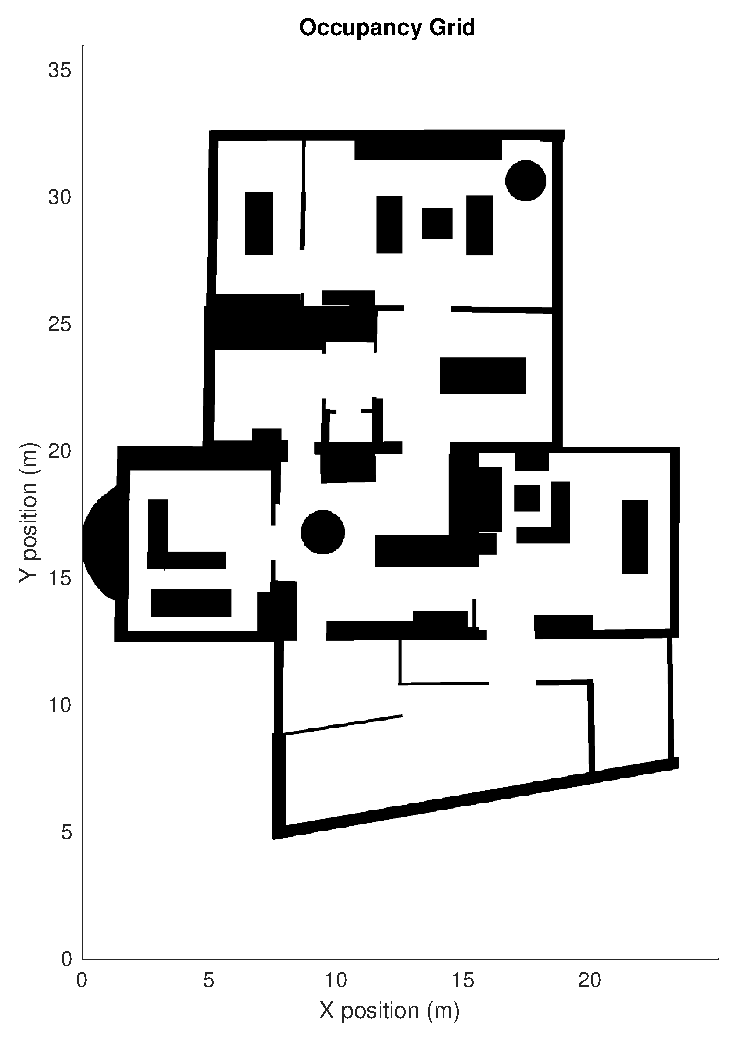
\includegraphics[width=0.4\linewidth]{images/20201030_1157_pf_map_1}
   	\caption{Particle Filter two dimensional probability function, where white and black has a probability of 1 and zero, respectively.}
   	\label{fig:pf_map}
   \end{figure}
   
	A map also indicates door locations, which are used as landmarks. If a door opening is detected through activity recognition, a conditional probability at each particle can be used to determine its weight, as 
	\begin{subequations}
		\begin{equation}
			c^*_{k}=\sum_{i=1}^{N} w_{k | k}^{i} p_{\scaleto{door}{4pt}}\left(y_{k} | x_{k}^{i}\right)
			\label{eq:pf_door_normalization}
		\end{equation}
		\begin{equation}
			\omega^{i*}_{k|k} = \frac{1}{c^*_k} \omega^i_{k|k} p_{\scaleto{door}{4pt}}(y_k|x^i_k),
			\label{eq:pf_door_weight}	
		\end{equation}
	\end{subequations}

 In the case of \cref{fig:pfdiagram}, if a door activity is detected the weight of particles P1 and P3 will be made higher than that of P2. This measurement update can only happen when a door interaction detection occurs, and happens after the map constraint measurement update.
	
	\begin{figure}[]
			\centering
			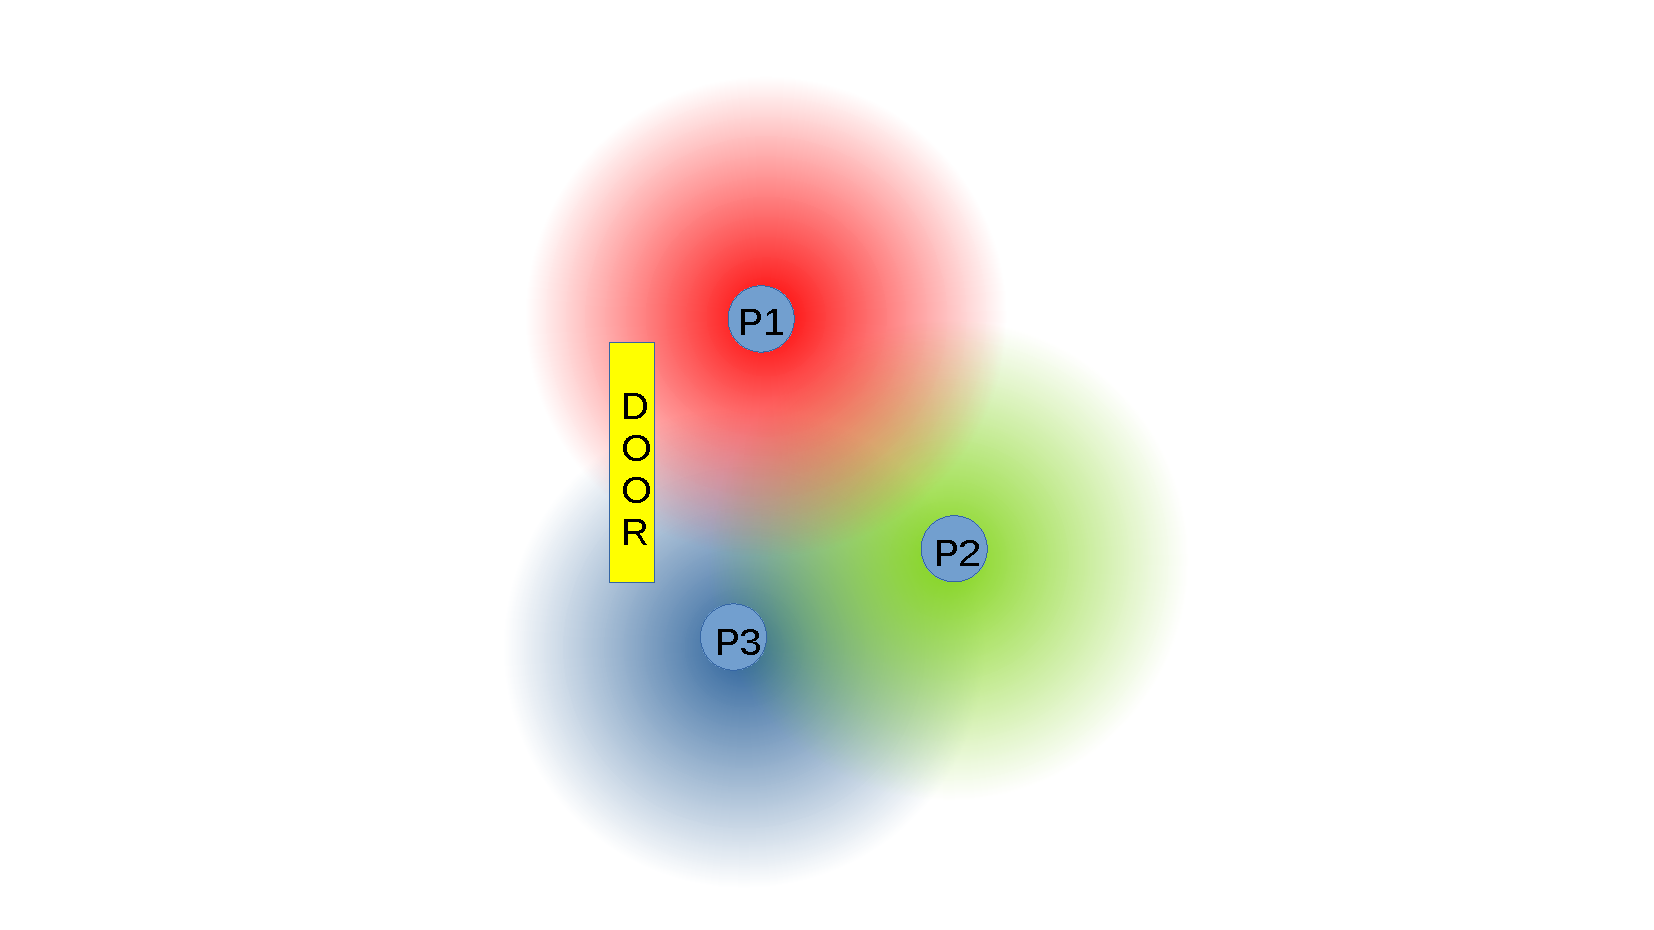
\includegraphics[trim=240 0 220 0, clip, width=0.35\linewidth]{images/pf_diagram}
			\caption{ Particles with a multivariate normal probability density function, represented by color gradient. At door interaction detection, particle weight is determined by probability at location of door in individual density functions.}
			\label{fig:pfdiagram}
	\end{figure}
	
	\item \textbf{Resampling}\\
	Resampling is used to select a new group of particles based on the weights of the current particles. The higher the weight of a particle is, the more likely it will be resampled. A particle can even be resampled multiple times. \par 
	There are multiple methods that can be used for resampling including multinomial, stratified, systematic, and	residual resampling \cite{hol2006resampling,gustafsson2010statistical}. \citet{hol2006resampling} conclude that  systematic resampling is the best considering resampling quality and computational complexity. Systematic resampling is defined as 
	
	\begin{align}
		x^{i*} &= x(F^{-1}(u^i)) \\
		u^i &= \frac{(i-1) + \tilde{u}}{N}, \tilde{u} \sim \mathcal{U}[0,1).
	\end{align}	
	
	 Here $x^{i*}$ represents the newly sample particle with index $i$, $F^{-1}$ represents the generalized inverse of the cumulative probability distribution of the normalized particle weights. Once the particles are resampled the particle weights are reset with $\omega^i_{k+1|k} = 1/N$ . \par
	Resampling inevitably destroys information and therefore increases uncertainty by the random sampling \cite{gustafsson2010particle}. Resampling should therefore occur only when it is needed. \citet{gustafsson2010statistical} proposes the use of  \textit{effective number of samples} to trigger a  resampling. This can be calculated as 
	\begin{subequations}
		\begin{equation}
		N_{\mathrm{eff}}=\frac{1}{\sum_{i=1}^{N}\left(w^{i}\right)^{2}},
		\end{equation}
		
		where
		
		\begin{equation}
		1 \leq N_{\mathrm{cff}} \leq N.
		\end{equation}
	\end{subequations}
	
	The resampling condition can then be defined as $N_{eff} < N_{th}$ \cite{gustafsson2010statistical}, where the threshold can be placed at $N_{th} = 2N/3$, with $N$ being the total number of particles.
	
	
	\item \textbf{Time update} \\	
	After resampling, the new particles update their state with a dynamic model. For indoor localization using a step and heading trajectory as input, the dynamic model used is
	
	\begin{equation}
		\label{eq:SHS_dynamic_model_with_noise}
		x^i_{k + 1}
		=
		\left(\begin{array}{l}
			p_{1,k}^i + (l_{k} + e_l) * \cos (\theta_{k}^i) \\
			p_{2,k}^i + (l_{t} + e_l) * \sin (\theta_{k}^i) \\
			\theta_{k}^i + \Delta \phi + e_\theta 
		\end{array}\right), \quad
		e_{\theta} \sim \mathcal{N}\left(0, \sigma_{\theta}^{2}\right), \quad e_{l} \sim \mathcal{N}\left(0, \sigma_{l}^{2}\right).
	\end{equation}

The inputs to this dynamic model are $l_{t}$, which is the step length found by step detection and step length estimation, and $\Delta \theta_t$, which is the change in heading between the current and previous timestep of the step and heading trajectory, found through the orientation estimation. These variables have additive zero mean Gaussian noise realizations $e_{\theta}$ and $e_{l}$, representing the uncertainty in the values of these inputs.
\end{enumerate}
The resulting particle filter from the previous steps is summarized in \cref{algo:bootstrap_PF}.

\begin{algorithm}[H]
	\small
	\SetAlgoLined
	\caption{Indoor Localization Particle Filter}
	\label{algo:bootstrap_PF}
	$i = 1,...,N$.   \\
	% choose a proposal distribution $ q(x_{k+1}|x_{1:k},y_{k+1})$, resampling strategy and the number of particles N.\\
	% \KwResult{Write here the result }
	\underline{Initialization:}\\
	choose the number of particles N.
	Generate initial distribution with
	\begin{subequations}
		\begin{equation}
			x^i_1 \sim p_{x_1},
		\end{equation}
		and let
		\begin{equation}
			\omega^i_{1|0} = 1/N.
		\end{equation}
	\end{subequations}
	
	\For{k = 1,2,...}{
		\underline{Measurement update:}\\
		\begin{subequations}
			\begin{align}
				\omega^i_{k|k} &= \frac{1}{c_k} \omega^i_{k|k-1} p_{\scaleto{map}{4pt}}(x^i_{k:k-1}),
				\label{eq:algo_pf_map_weight}\\	
				c_{k} &=\sum_{i=1}^{N} w_{k | k-1}^{i} p_{\scaleto{map}{4pt}}\left( x^i_{k:k-1}\right)
				\label{eq:algo_pf_map_normalization}
			\end{align}
			\label{pf_map_update}
		\end{subequations}
		
		
		\begin{subequations}
			
			\If{(door interaction detected)}{
				\begin{align}
					c_{k}&=\sum_{i=1}^{N} w_{k | k}^{i} p_{\scaleto{door}{4pt}}\left(y_{k} | x_{k}^{i}\right)
					\label{eq:pf_door_normalization} \\			
					\omega^i_{k|k} &= \frac{1}{c_k} \omega^i_{k|k} p_{\scaleto{door}{4pt}}(y_k|x^i_k),
					\label{eq:pf_door_weight}	
				\end{align}
			}
			\label{eq:pf_door_update}			
		\end{subequations}\smallskip
		
		
		\underline{Resampling:}\\
		\begin{subequations}
			\begin{equation}
				N_{\mathrm{eff}}=\frac{1}{\sum_{i=1}^{N}\left(w^{i}\right)^{2}},
			\end{equation}
			\If{	$N_{\mathrm{eff}} < 2N/3$}{
				
				\begin{align}
					x^{i*} &= x(F^{-1}(u^i)) \\
					u^i &= \frac{(i-1) + \tilde{u}}{N}, \tilde{u} \sim \mathcal{U}[0,1).\\
					\omega^i_{k+1|k} &= 1/N
				\end{align}
				
				\label{eq:pf_resampling}	
		}	\end{subequations}\smallskip
		\underline{Time update:}\\
		\begin{equation}
			\label{eq:algo_SHS_dynamic_model_with_noise}
			x^i_{k + 1}
			=
			\left(\begin{array}{l}
				p_{1,k}^i + (l_{k} + e_l) * \cos (\theta_{k}^i) \\
				p_{2,k}^i + (l_{t} + e_l) * \sin (\theta_{k}^i) \\
				\theta_{k}^i + \Delta \phi + e_\theta 
			\end{array}\right), \quad
			e_{\theta} \sim \mathcal{N}\left(0, \sigma_{\theta}^{2}\right), \quad e_{l} \sim \mathcal{N}\left(0, \sigma_{l}^{2}\right).
		\end{equation}		
	}
\end{algorithm}
\newpage

\textbf{State Estimation}\\
The Particle Filter is able to estimate non linear posterior densities, allowing for multimodal distributions \cite{gustafsson2010particle,kihlberg2012map}. Multimodal distribution refers to distributions with multiple maxima in the probability density function. This allows the particle filter to have multiple hypotheses for the system that it is modeling. In the case of localization, this translates to indicating that there are two position estimates that are equally as likely based on the information that the filter has received so far. This can occur due to symmetry in the indoor environment \cite{Woodman2008}.

The posterior distribution is the primary output of a particle filter \cite{gustafsson2010particle}. For state inference purposes a single point estimate is more convenient \cite{Saha2009}. The weights and positions of the particle cloud can be used to generate a single point estimate \cite{gustafsson2010particle}. There are different ways of defining the eventual position estimate. The maximum a posteriori (MAP) estimate picks the particle with the highest weight from the posterior distribution \cite{Saha2009}, while the  minimum mean square error (MMSE) estimate calculates a weighted mean \cite{gustafsson2010particle,Saha2009}.\par 

For the particle filter method outlined in this thesis, both forms have disadvantages.
Firstly, MMSE does not work well in situations in which there are multiple equal likely hypotheses \cite{Saha2009}. In such a case it will take the position in between the different hypothesis as the position estimate. A good example of this can be found in \cref{fig:lopen_11_mmse_estimator}. The figure shows the output of a particle filter after 10 time steps. There are clear groups visible, all moving in different directions. The position estimate is expected to be in either one of the particle clouds, however RMSE put it between the different clouds, a position in which no particles are found, making it a subpar estimate. \par 
Implementing MAP as the state estimate in the particle filter is actually similar to MMSE. The measurement update that occurs every timestep of the step and heading trajectory is the one that compares particle trajectories to map constraints, setting infeasible particles probability to zero and feasible particles to one. All feasible particles will then have the same weighting. Since all particles have the same weight, a MAP cannot be defined.
\begin{figure}[]
	\centering
	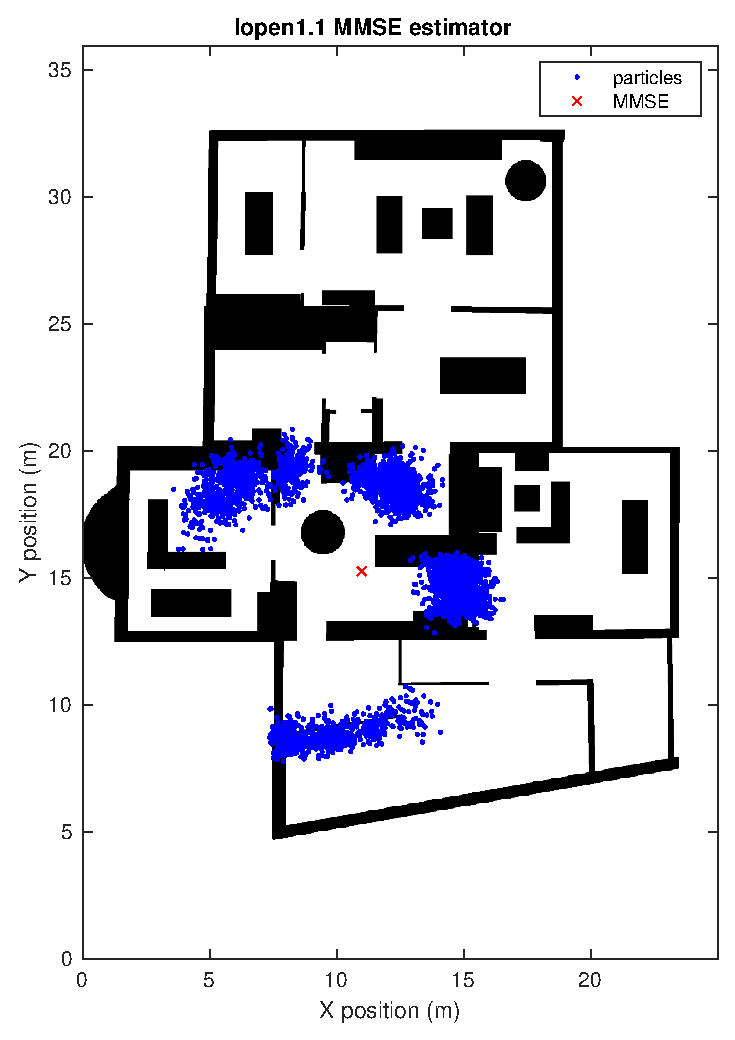
\includegraphics[width=0.35\linewidth]{images/20201108_1751_lopen1_1_MMSE_estimator}
	\setlength{\belowcaptionskip}{-20pt}
	\caption{Particle filter after 10 iterations, showing how MMSE does not provide a suitable single point estimate.}
	\label{fig:lopen_11_mmse_estimator}
\end{figure}

A different approach is to using the particles at the last timestep of the SHS trajectory and calculate all ancestors of these particles. A final particle with all its ancestors generate a feasible trajectory.  Averaging the trajectories of multiple final particles can give an estimate trajectory within the indoor environment.

\section{Activity Recognition}
\label{sec:method-AR}

Activity recognition is large research field in which methods span a broad range of complexity, from simple thresholding to the use of deep learning techniques such as neural networks and its many variations \cite{Lima2019}. Even the subset of activity recognition that use IMU sensors does not decrease the amount of possibilities significantly.

%TODO add drear as activity recognition

The choice for a particular activity recognition method is often a trade-off between performance and computational complexity \cite{Bulling2014}. Considering the scope of this thesis, certain constraints can be applied, such as that the system should be able to function on a smartphone and must use comparable sensors to those found in such devices, thus MEMS IMUs. \citet{Shoaib2015} have performed an extensive survey that focuses on the online activity recognition solely using mobile phone sensors and onboard processing. Other metrics such as resource consumption were also presented. 30 papers were found to meet the requirements of the review. Within the review they indicate that most commonly used classification methods include Decision Tree, support vector machine (SVM), K-nearest neighbor (KNN) and Naive Bayes, in descending order. A third of the papers were found to use decision trees. All but 6 of the papers had the training process occurring offline. The classification process takes the method generated offline, and uses it online to classify new activities. The authors refrain from listing any performance measures, such as accuracy or precision, since no direct comparison between the different methods is made. \citet{Ahmad2020} specifically focuses on seeing whether smartphone activity recognition techniques are also applicable to smartwatches, and what parameters, including classifiers, work best. Activities to recognize included walking, up-stairs, down-stairs, running, and jogging. Their results indicated that  Decision Trees, SVM and KNN had around 90 percent accuracy a minor difference. \citet{Shoaib2016} show that combining information from both a smartwatch and smartphone, complex human activity recognition is improved compared to when only a smart watch is used. 


\textcolor{purple}{ section overview:
\begin{itemize}
	\item Many different type of activity recognition methods, from simple to complex. 
	\item Depends on what needs to be detected. For activities with a clear time based foot print, simple method can be good enough. It is possible to construct own decision tree.
	\item \cref{fig:stand_still_detection_from_shs} shows ground truth first door interaction and the accelerometer traces from a smartwatch and a standstill detection from SHS.
	\item standstill detection from SHS is made by determining when the period buildup between steps exceeds over 3 seconds.
	\item A simple manually constructed decision tree can be used to indicate door interaction. Using both smartwatch data and shs standstill detection the system can distinguish between standing still and interaction with a door.  
\end{itemize}}

\begin{figure}[H]
	\centering
	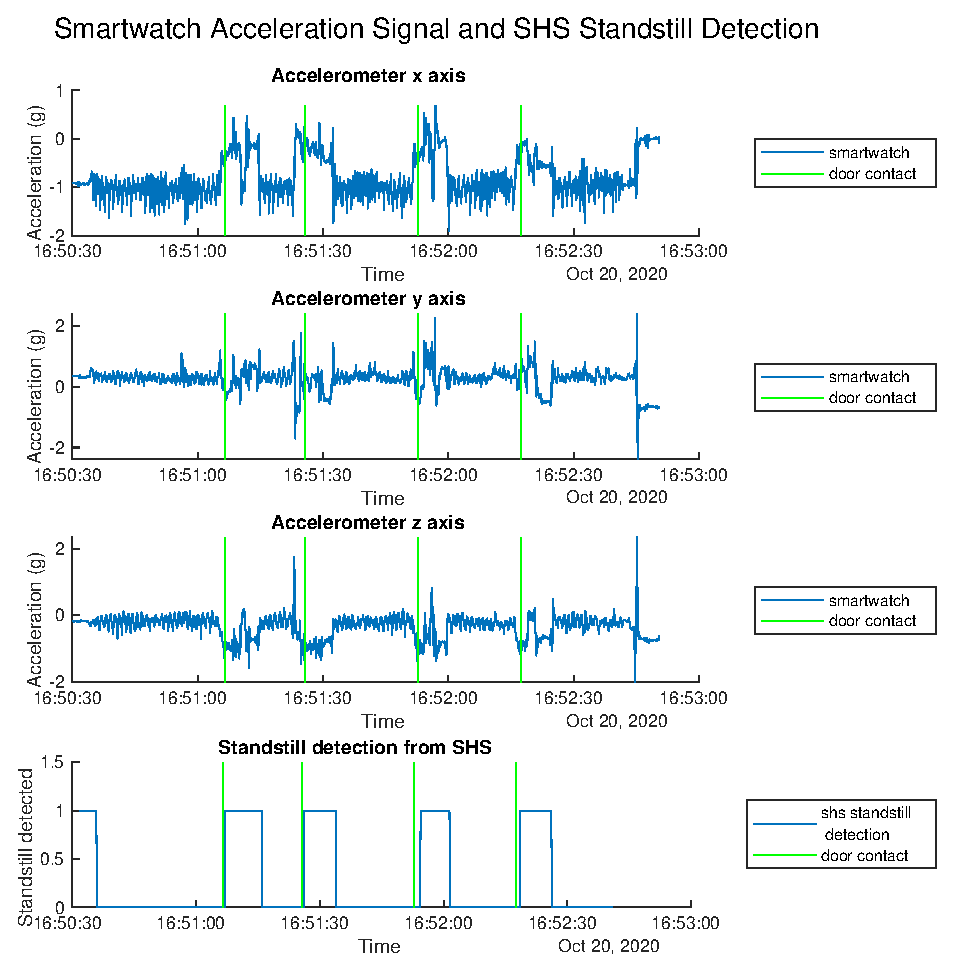
\includegraphics[width=0.7\linewidth]{images/20201103_1325_Standstill_detection_from_SHS}
	\caption{Smartwatch accelerometer data and SHS stand still detection}
	\label{fig:stand_still_detection_from_shs}
\end{figure}

\begin{figure}[H]
	\centering
	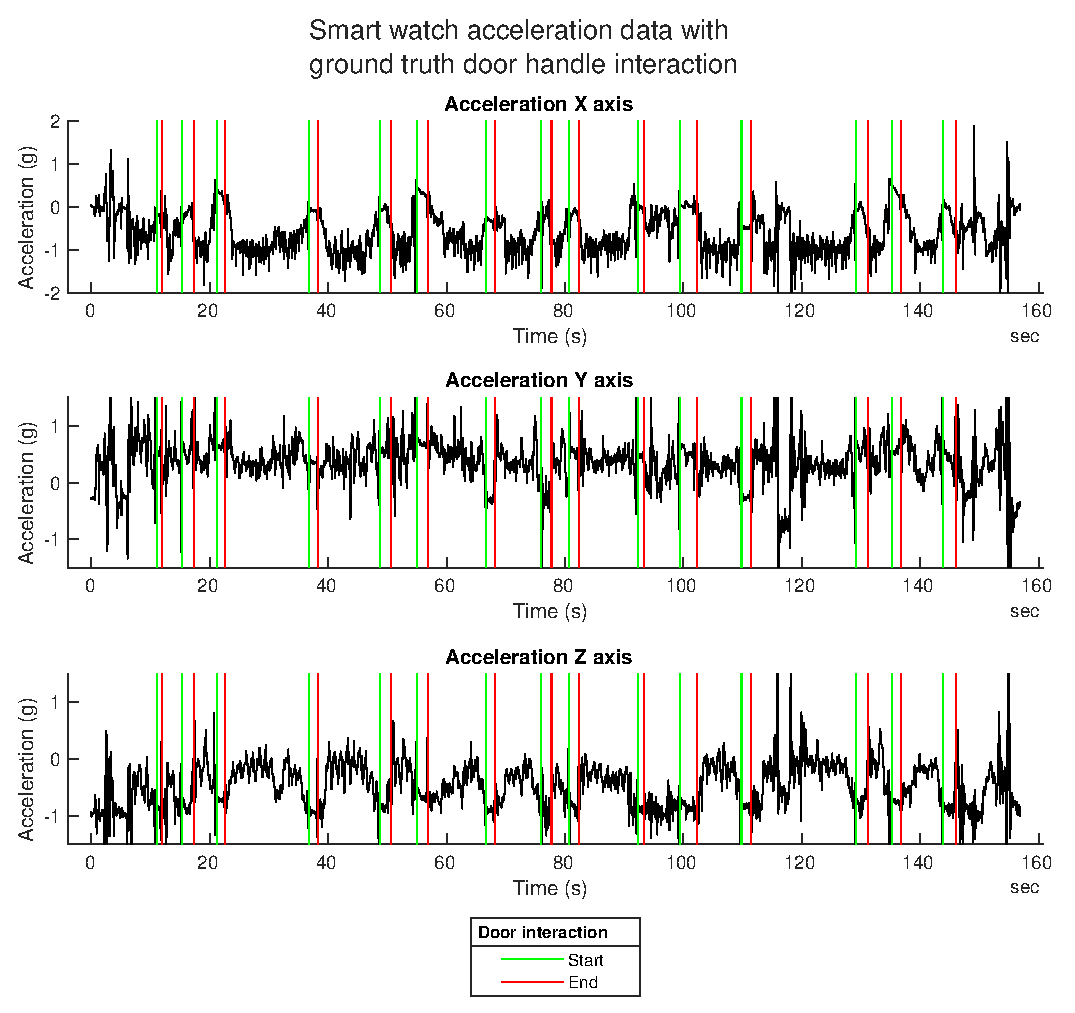
\includegraphics[width=0.7\linewidth]{images/20201114_1820_smartwatch_acc_with_gt_door_and_door_detect_1}
	\caption{}
	\label{fig:202011141820smartwatchaccwithgtdooranddoordetect1}
\end{figure}

\begin{figure}[H]
	\centering
	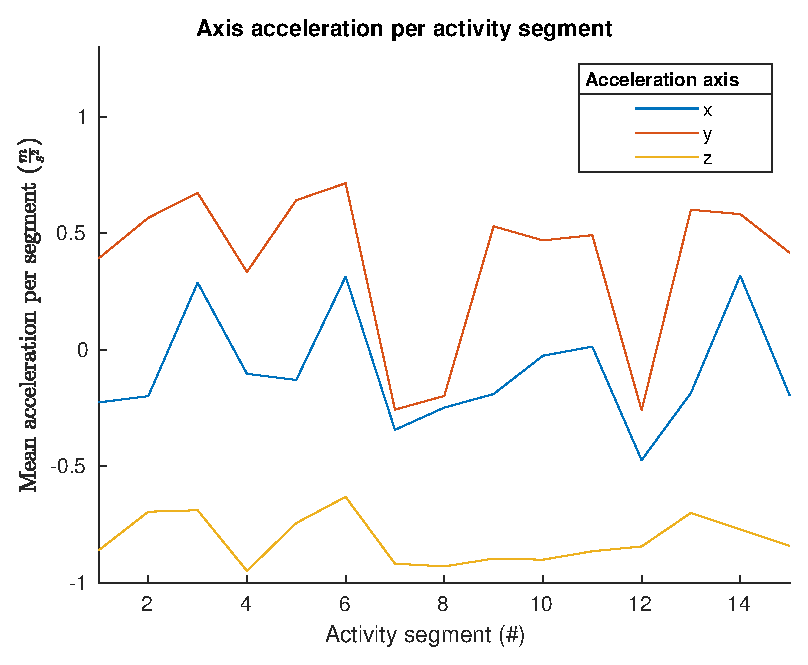
\includegraphics[width=0.7\linewidth]{images/20201114_1858_Axis_acceleration_per_activity_segment}
	\caption{}
	\label{fig:202011141858axisaccelerationperactivitysegment}
\end{figure}

\begin{figure}[H]
	\centering
	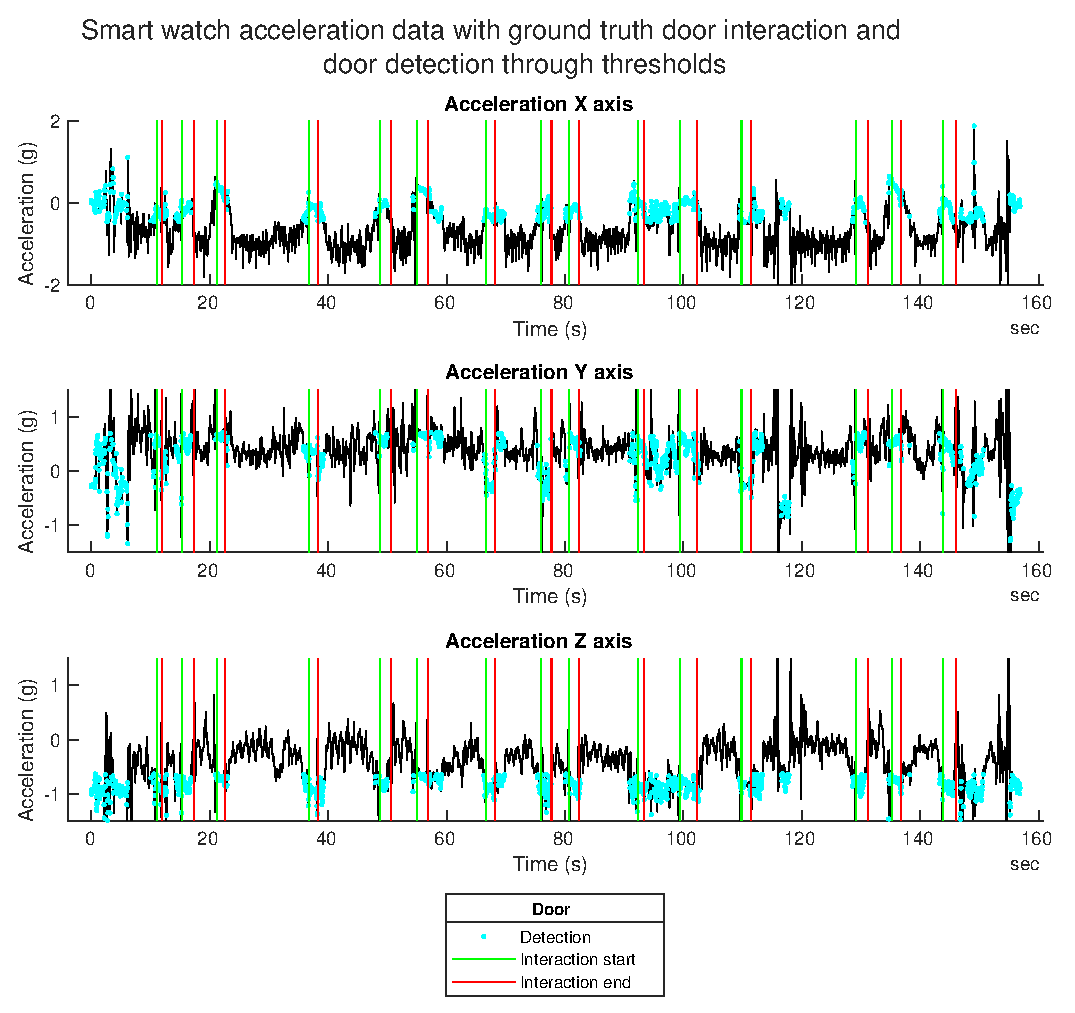
\includegraphics[width=0.7\linewidth]{images/20201114_1820_smartwatch_acc_with_gt_door_and_door_detect_2}
	\caption{}
	\label{fig:202011141820smartwatchaccwithgtdooranddoordetect2}
\end{figure}

\textcolor{red}{I have more data on smartwatch accelerometer also from different people. I can use that data to determine the threshold on accelerometer data that would work on different people. Do you think that this is a good idea?}